% Generated by book/tools/notebook_to_tex.py. Do not edit by hand.

\chapter[작은 BERT 이진 분류 (Yelp)]{작은 BERT 이진 분류 (English Yelp Fine-tuning)}

\label{ch:21}

\markboth{작은 BERT 이진 분류 (Yelp)}{작은 BERT 이진 분류 (Yelp)}

\chaptermeta{21_en_bert_classify/21_en_bert_classify.ipynb}{https://colab.research.google.com/github/yoon-gu/neuqes-101/blob/master/21_en_bert_classify/21_en_bert_classify.ipynb}{20장에서 사전학습한 작은 BERT 본체를 Yelp 이진 분류로 파인튜닝}



\index{1BERT fine tuning@BERT fine-tuning}

\index{1BertForSequenceClassification@BertForSequenceClassification}

\index{1Yelp polarity@Yelp polarity}

\index{1binary classification@binary classification}

\index{1CrossEntropyLoss@CrossEntropyLoss}

\index{1classification head@classification head}

\index{1transfer learning@transfer learning}

\index{1DistilBERT comparison@DistilBERT comparison}

\index{1confusion matrix@confusion\_matrix}

\index{1classification report@classification\_report}

\index{1roc auc score@roc\_auc\_score}

\index{0이진 분류@이진 분류}

\index{0파인튜닝@파인튜닝}

\index{0전이 학습@전이 학습}

\index{0분류 헤드@분류 헤드}

\index{0혼동 행렬@혼동 행렬}

\index{0전이 성능@전이 성능}

\index{1load state dict@load\_state\_dict}

\index{1classifier head@classifier head}

\index{1single label classification@single\_label\_classification}

\index{1softmax@softmax}

\index{1fine tune loss@fine-tune loss}

\index{1Yelp binary classification@Yelp binary classification}

\index{1GLUE@GLUE}

\index{1domain transfer@domain transfer}

\index{1DAPT@DAPT}

\index{1random baseline@random baseline}

\index{1head replacement@head replacement}

\index{1body weight transfer@body weight transfer}

\index{0본체 가중치@본체 가중치}

\index{0헤드 교체@헤드 교체}

\index{0도메인 전이@도메인 전이}

\index{0일반 도메인 사전학습@일반 도메인 사전학습}

\index{0태스크 도메인@태스크 도메인}

\index{0정확도@정확도}

\index{1AUC@AUC}



\section{변화추적표}

\begin{booktable}{21장 변화추적표}{tab:ch21-01}
\begin{adjustbox}{max width=\textwidth}
\begin{tabular}{@{}lllllll@{}}
\toprule
Ch & 모델 & 토크나이저 & 데이터 & Output Head & Activation & Loss \\
\midrule

10 & DistilBERT 파인튜닝 (약 66M) & \inlinecode{bert-base-uncased} WordPiece & Yelp 이진 (4-5 \(\to\) 1, 1-2 \(\to\) 0) & \inlinecode{Linear(H,\ 1)} & sigmoid & \inlinecode{BCEWithLogitsLoss} \\
18 & klue/bert-base + 보조 & WordPiece (한국어, 사전학습) & KLUE-YNAT 합성 + 보조 라벨 & 메인(7) + 보조 & sigmoid + 태스크별 & \inlinecode{BCEWithLogitsLoss\ +\ λ·L\_aux} \\
19 & --- (토크나이저 학습 전용) & WordPiece + WordLevel (둘 다 직접 학습) & Yelp text + NSMC text & --- & --- & --- \\
20 & 작은 BERT (직접, scratch) & \inlinecode{bert-base-uncased} 토크나이저 (가져옴) & Wikitext-103 paragraphs (일반 도메인) & MLM head & softmax (MLM) & \inlinecode{CrossEntropyLoss} (masked token) \\
\textbf{21 \(\leftarrow\) 여기} & \textbf{\ref{ch:20}장 사전학습 BERT + 분류 헤드 (약 10M)} & (\ref{ch:20}장과 동일) & \textbf{Yelp 이진화 (다른 도메인 transfer)} & \textbf{\inlinecode{Linear(H,\ 2)}} & \textbf{softmax} & \textbf{\inlinecode{CrossEntropyLoss}} \\
22 (다음) & 작은 BERT (직접, scratch) --- 한국어 & \inlinecode{klue/bert-base} 토크나이저 (가져옴) & 한국어 Wikipedia paragraphs (일반 도메인) & MLM head & softmax (MLM) & \inlinecode{CrossEntropyLoss} (masked token) \\
\bottomrule
\end{tabular}
\end{adjustbox}
\end{booktable}

전체 장 표는 \href{https://github.com/yoon-gu/neuqes-101\#챕터별-변화추적표}{루트 README.md}를 참고하세요.

\textbf{Phase 3 안에서의 위치} --- \ref{ch:19}장 (토크나이저 학습) \(\to\) \ref{ch:20}장 (모델 사전학습) \(\to\) \textbf{\ref{ch:21}장 (분류 fine-tune)} \(\to\) \ref{ch:22}장 (한국어 사전학습) \(\to\) \ref{ch:23}장 (한국어 분류). \ref{ch:21}장이 Phase 3 의 \emph{영어 절반 마무리} --- \ref{ch:10}장 비교가 클라이맥스.



\section{변경점: \ref{ch:20}장 대비}

\begin{booktable}{21장 변경점 요약}{tab:ch21-02}
\begin{adjustbox}{max width=\textwidth}
\begin{tabular}{@{}lll@{}}
\toprule
축 & \ref{ch:20}장 (작은 BERT scratch MLM, 위키) & \ref{ch:21}장 (작은 BERT 분류 fine-tune, Yelp) \\
\midrule

\textbf{이 장의 task} & MLM 사전학습 (masked token 예측) & \textbf{이진 분류 (긍정/부정)} \(\leftarrow\) \emph{task 축 변화} \\
모델 클래스 & \inlinecode{BertForMaskedLM} & \textbf{\inlinecode{BertForSequenceClassification(num\_labels=2)}} \\
본체 (embedding + encoder) & random init \(\to\) MLM 학습 & \textbf{\ref{ch:20}장 사전학습 본체 그대로 이어받음} \\
출력 헤드 & MLM head (vocab 30,522 차원) & \textbf{분류 head (\inlinecode{Linear(256,\ 2)})} \(\leftarrow\) 새 random init \\
토크나이저 & \inlinecode{bert-base-uncased} (vocab 30,522) & (그대로) \\
\textbf{데이터} & \textbf{Wikitext-103 paragraphs (일반 도메인, 라벨 없음)} & \textbf{Yelp 이진 (다른 도메인, 라벨 사용)} \(\leftarrow\) \emph{사전학습과 fine-tune 도메인이 다름} \\
Loss & \inlinecode{CrossEntropyLoss} (vocab 30,522 logits) & \textbf{\inlinecode{CrossEntropyLoss} (2 logits)} \(\leftarrow\) K 만 큰 변화 \\
학습률 & 5e-4 (scratch 사전학습) & \textbf{2e-5} (fine-tune, 표준) \\
\bottomrule
\end{tabular}
\end{adjustbox}
\end{booktable}

\begin{quote}
\textbf{변경점 한 가지 원칙} --- Phase 3 안에서 \emph{task 축} 이 변합니다 (MLM \(\to\) 분류). 데이터 \emph{도메인} 도 같이 변합니다 (위키 \(\to\) Yelp) --- 이게 \emph{진짜 transfer 의 본질}. 모델 본체·토크나이저는 그대로, 헤드와 라벨 형식·데이터 도메인이 바뀝니다. 이게 \emph{사전학습-fine-tune 패러다임} 의 핵심: 본체는 한 번 학습한 \emph{일반 표상} 을 재사용, downstream task 도메인마다 \emph{작은 헤드 + 작은 학습률} 로 적응.
\end{quote}

\subsection{두 데이터셋의 역할}

본 장의 특수성 --- 한 노트북에 두 데이터셋이 함께 들어갑니다.

\begin{booktable}{21장 두 데이터셋의 역할 표}{tab:ch21-03}
\begin{adjustbox}{max width=\textwidth}
\begin{tabular}{@{}lll@{}}
\toprule
단계 & 데이터셋 & 용도 \\
\midrule

3 §MLM 사전학습 & \inlinecode{Salesforce/wikitext}, \inlinecode{wikitext-103-raw-v1} 2K paragraphs \(\times\) 3 epoch & self-supervised MLM (라벨 없음, 일반 위키 본문) \\
4-5 §분류 fine-tune & \inlinecode{fancyzhx/yelp\_polarity} 5K/1K & supervised 이진 분류 (긍정/부정 라벨) \\
\bottomrule
\end{tabular}
\end{adjustbox}
\end{booktable}

같은 토크나이저 (\inlinecode{bert-base-uncased}) 가 두 데이터셋의 모든 텍스트를 처리. 본체가 \emph{위키 일반 어휘} 로 사전학습된 표상이 \emph{Yelp 리뷰(식당·업체) 도메인 토큰} 에 얼마나 잘 전이되는가가 본 장의 측정 대상.

\subsection{\texorpdfstring{\ref{ch:10}장 (DistilBERT) 과의 비교가 본 장의 메인 메시지 --- 이제 \emph{fair}}{\ref{ch:10}장 (DistilBERT) 과의 비교가 본 장의 메인 메시지 --- 이제 fair}}

\begin{booktable}{21장 10장 (DistilBERT) 과의 비교가 본 장의 메인 메시지 - 이제 fair 표}{tab:ch21-04}
\begin{adjustbox}{max width=\textwidth}
\begin{tabular}{@{}llll@{}}
\toprule
차원 & \ref{ch:10}장 (DistilBERT) & \ref{ch:21}장 (이 장) & 비고 \\
\midrule

본체 파라미터 & 약 66M & \textbf{약 10M} & \ref{ch:21}장은 1/6 작음 \\
사전학습 코퍼스 & Wikipedia + BookCorpus (약 33억 토큰, 일반 도메인) & \textbf{Wikitext-103 paragraphs 2K (약 27만 토큰, 일반 도메인)} & 약 1.2만배 격차, \textbf{둘 다 일반 위키} \\
사전학습 시간 & TPU 수일 (대규모 인프라) & \textbf{T4 약 15초} (2K \(\times\) 3 epoch = 198 step) & \\
Fine-tune 도메인 & Yelp 이진 (사전학습과 다른 도메인) & Yelp 이진 (사전학습과 다른 도메인) & \textbf{둘 다 일반 \(\to\) Yelp transfer 라 fair} \\
분류 fine-tune 셋업 & \ref{ch:10}장 = 이 장 동일 (같은 데이터, 같은 hyperparams) & & 변하는 건 \emph{본체 출발점} 뿐 \\
실측 accuracy & 약 0.90 & \textbf{random (0.50) 과 \ref{ch:10}장의 중간쯤} & 실행마다 흔들려 본문에 못 박지 않습니다 --- 값은 §6 의 비교 셀 출력 \\
\bottomrule
\end{tabular}
\end{adjustbox}
\end{booktable}

비교가 \emph{공정} 한 이유 --- \ref{ch:10}장도 본 장도 둘 다 \emph{일반 도메인 위키 사전학습 \(\to\) Yelp 분류 transfer} 의 같은 패턴. \emph{사전학습 규모} (약 1.2만배) 와 \emph{모델 크기} (약 6배) 만 차이. 만약 \ref{ch:21}장이 Yelp text 로 사전학습했다면 비교가 unfair 했을 것 --- domain-adaptive pretraining 우위 때문.

이 격차가 \emph{사전학습 규모의 가치} 를 정량으로 보여줍니다. 한편 \emph{작은 일반 도메인 사전학습이 random init 보다 나은가}, \emph{같은 GPU compute 를 fine-tune 에 모두 쏟으면 그 차이가 메워지는가} 는 이 노트북에서 측정하지 않습니다 --- 부록 노트북 \href{https://colab.research.google.com/github/yoon-gu/neuqes-101/blob/master/21_en_bert_classify/appendix_compute_budget.ipynb}{\inlinecode{appendix\_compute\_budget.ipynb}} 이 그 비교를 위한 셋업입니다. \textbf{부록의 답은 이 규모에서 \textquotesingle 메워진다\textquotesingle{} 입니다} --- random init 대비 순 효과는 수 \%p 로 실재하지만, 같은 GPU 예산을 분류 fine-tune 에 쓰는 쪽이 더 크게 이깁니다. \emph{사전학습의 가치는 규모에서 나온다} 는 이 장의 메시지를 반대쪽에서 받쳐 줍니다.



\section{\texorpdfstring{Loss 함수의 변화 --- MLM CE (vocab=30,522) \(\to\) 분류 CE (K=2)}{Loss 함수의 변화 --- MLM CE (vocab=30,522) \textbackslash to 분류 CE (K=2)}}

\ref{ch:20}장의 MLM 도 본질은 \emph{vocab 위에서의 다중 분류} 였습니다. 다만 K = vocab\_size = 30,522 라 어려운 task. 이 장은 K = 2 의 \emph{훨씬 쉬운} 분류 task.

\subsection{수식}

분류 task 의 CE 는 \ref{ch:11}장과 같습니다 (K=2):

\begin{equation}
\label{eq:ch21-01}
L_{\text{cls}} = -\frac{1}{N}\sum_{i=1}^{N} \log \hat p_{i, y_i}
\end{equation}

식~\eqref{eq:ch21-01}은 이 절에서 사용하는 핵심 관계를 정리한 것입니다.

\begin{itemize}
\tightlist
\item
  \(\hat p_{i, k} = \mathrm{softmax}(z_i)_k\) --- K=2 차원 softmax
\item
  \(y_i \in \{0, 1\}\) --- 정수 라벨
\end{itemize}

\subsection{두 CE 기준선 비교}

\begin{booktable}{21장 두 CE 기준선 비교 표}{tab:ch21-05}
\begin{adjustbox}{max width=\textwidth}
\begin{tabular}{@{}llll@{}}
\toprule
task & K & random baseline loss \(\log K\) & 학습 어려움 \\
\midrule

MLM (\ref{ch:20}장) & 30,522 & \textbf{10.33} & 매우 어려움 --- 가려진 토큰 자리에 \emph{vocab 전체 후보} 중 정답을 \\
분류 (\ref{ch:21}장) & 2 & \textbf{0.693} & 상대적으로 쉬움 --- 긍정/부정 둘 중 하나 \\
\bottomrule
\end{tabular}
\end{adjustbox}
\end{booktable}

학습 첫 step 의 loss 가 약 0.693 부근이면 모델이 \emph{균등 추측} 단계. fine-tune 첫 step 에서 분류 헤드만 새로 init 됐으므로 \emph{이 정도} 가 정상.

\subsection{\texorpdfstring{사전학습 효과와 loss 곡선}{사전학습 효과가 loss 곡선 에 어떻게 드러나나}}

\begin{booktable}{21장 사전학습 효과가 loss 곡선 에 어떻게 드러나나 표}{tab:ch21-06}
\begin{adjustbox}{max width=\textwidth}
\begin{tabular}{@{}llll@{}}
\toprule
셋업 & 학습 첫 step loss & 학습 종료 loss (epoch 2) & 메모 \\
\midrule

random init + 분류 (부록) & 약 0.693 & \textbf{약 0.69} (\inlinecode{executed/appendix\_compute\_budget.ipynb} 셋업 C 기록) & 본체도 분류 헤드도 random --- 2 epoch 으로는 기준선을 거의 못 벗어남 \\
Wikitext-103 MLM 사전학습 본체 + 분류 (메인) & 약 0.693 & \textbf{랜덤 기준선 바로 아래} --- 값은 §5-1 학습 곡선 셀 출력 & 2K \(\times\) 3 epoch 은 아주 얕은 사전학습이라, 2 epoch fine-tune 으로 기준선에서 크게 내려가지 못합니다 \\
\ref{ch:10}장 DistilBERT 사전학습 본체 + 분류 & 약 0.693 & \textbf{약 0.16} (\inlinecode{executed/10\_bert\_binary\_sigmoid.ipynb}, 커밋 \inlinecode{d9fc77c} 기록) & 대규모 일반 도메인 사전학습이 만든 표상의 위력 \\
\bottomrule
\end{tabular}
\end{adjustbox}
\end{booktable}

random baseline 은 \emph{세 셋업 모두 같음} --- 사전학습은 \emph{학습 속도} 와 \emph{수렴점} 에 영향을 줍니다. 다만 이 장의 사전학습은 \emph{2K paragraphs \(\times\) 3 epoch} 으로 아주 얕아서, 종료 loss 가 랜덤 기준선(0.693)을 크게 밑돌지는 못합니다. \emph{얼마나 내려가는지} 는 실행마다 흔들리므로 본문에서 숫자를 못 박지 않고 §5-1 의 곡선과 §6 의 셀 출력을 단일 출처로 둡니다. random init 과의 직접 비교는 부록에서 다룹니다 --- 부록 실측에서 메인 조건(A)이 random init(C)보다 조금 앞섰지만, 같은 GPU 예산을 fine-tune 에 더 쓴 셋업(B)에는 뒤졌습니다.

\begin{quote}
\textbf{숫자로 감 잡기} (K=2, 정답 = 클래스 1):
\textbar{} logits \((z_0, z_1)\) \textbar{} softmax \(\to\) \(\hat p_1\) \textbar{} 손실 \textbar{}
\textbar-\/-\/-\textbar-\/-\/-\textbar-\/-\/-\textbar{}
\textbar{} (0, 0) \textbar{} 0.5 \textbar{} \textbf{0.693} \(\leftarrow\) random \textbar{}
\textbar{} (-1, +1) \textbar{} 0.881 \textbar{} 0.127 \textbar{}
\textbar{} (-2, +2) \textbar{} 0.982 \textbar{} 0.018 \textbar{}
\textbar{} (+2, -2) \textbar{} 0.018 \textbar{} \textbf{4.018} \(\leftarrow\) 자신 있게 틀림 \textbar{}
\end{quote}



\section{토크나이저 노트}

\ref{ch:20}장과 \emph{완전히 동일} --- \inlinecode{AutoTokenizer.from\_pretrained("bert-base-uncased")}, vocab 30,522 영어 WordPiece. 사전학습-fine-tune 패러다임의 핵심: \textbf{토크나이저는 사전학습부터 분류까지 전 구간에서 동일} 해야 함. 그래야 본체가 학습한 토큰 임베딩이 그대로 의미를 유지.

\subsection{위키와 Yelp 어휘}

본 장의 두 데이터셋이 \emph{같은 토크나이저} 를 공유하지만 \emph{어휘 분포} 는 꽤 다릅니다.

\begin{itemize}
\tightlist
\item
  \textbf{Wikitext-103 (MLM 사전학습)}: 일반 위키 어휘 --- 지명·인명·과학·역사 용어 (\inlinecode{capital}, \inlinecode{theorem}, \inlinecode{dynasty}, \inlinecode{proton} ...) 가 풍부. 격식 있는 문장 구조.
\item
  \textbf{Yelp polarity (분류 fine-tune)}: 영화 리뷰 어휘 --- 감성 형용사·구어체 (\inlinecode{amazing}, \inlinecode{terrible}, \inlinecode{loved}, \inlinecode{awful} ...) 가 풍부. 비격식 구어체.
\end{itemize}

같은 \inlinecode{bert-base-uncased} vocab (Wiki + BookCorpus 학습) 이 두 도메인을 \emph{모두} 합리적으로 커버 --- \emph{위키 본문} 의 격식 어휘는 본 장 사전학습이 직접 본 분포, \emph{Yelp 감성 어휘} 는 fine-tune 단계에서 본체가 적응. \emph{토크나이저는 운명공동체} 라 vocab 미스매치가 없습니다.

\subsection{분류 task 에서 {[}CLS{]} 토큰의 의미}

MLM 사전학습 (\ref{ch:20}장) 에서는 \inlinecode{group\_texts} 패턴으로 \emph{특수 토큰 없이} 토큰 스트림을 잘랐습니다. 분류 fine-tune 에서는 \emph{문장 단위} 입력이라 표준 BERT 포맷:

\Needspace{5\baselineskip}
\begin{lstlisting}
[CLS] the food was excellent and the service was great [SEP]
\end{lstlisting}

\begin{itemize}
\tightlist
\item
  \texttt{{[}CLS{]}} 의 최종 hidden state \(h_{[CLS]} \in \mathbb{R}^{256}\) 가 \emph{문장 표상}. 분류 헤드 \inlinecode{Linear(256,\ 2)} 가 이 위에 얹힘.
\item
  MLM 학습 중에는 \texttt{{[}CLS{]}} 의 hidden 이 \emph{암묵적} 으로만 학습됨 (옆 토큰들과 attention 공유). 분류 fine-tune 단계에서 \emph{이 자리} 가 본격 활용.
\end{itemize}

\subsection{헤드 교체와 파라미터}

\begin{booktable}{21장 헤드 교체와 파라미터 표}{tab:ch21-07}
\begin{adjustbox}{max width=\textwidth}
\begin{tabular}{@{}lll@{}}
\toprule
모델 부분 & \ref{ch:20}장 학습 끝 \(\to\) \ref{ch:21}장 시작 & 운명 \\
\midrule

임베딩 (vocab 30,522 \(\times\) hidden 256) & Wikitext-103 사전학습으로 \emph{일반 위키 어휘 표상} 학습 & \textbf{그대로 이어받음} (Yelp 어휘도 같은 vocab 안에 있어 호환) \\
Encoder 4 layer (attention + FFN) & MLM 으로 \emph{문맥 의존 표상} 학습 & \textbf{그대로 이어받음} \\
MLM head (\inlinecode{cls.predictions}) & vocab 위 분류 헤드 & \textbf{버려짐} \\
분류 head (\inlinecode{classifier}, \inlinecode{Linear(256,\ 2)}) & (없었음) & \textbf{새로 random init} \(\leftarrow\) Yelp fine-tune 으로 학습 \\
\bottomrule
\end{tabular}
\end{adjustbox}
\end{booktable}

\begin{quote}
\ref{ch:10}장의 DistilBERT 가 같은 흐름 (일반 도메인 MLM 사전학습 \(\to\) Yelp 분류 fine-tune) 을 \emph{큰 규모} 로 거친 결과. 우리도 같은 흐름을 \emph{작은 규모} 로 직접 거칩니다 --- 둘 다 \emph{위키 \(\to\) Yelp transfer} 라 비교가 fair.
\end{quote}



\section{환경 준비}



\textbf{baseline VRAM} (CUDA 환경에서만 의미 있는 출력 --- Colab T4 기준):



\Needspace{5\baselineskip}
\begin{lstlisting}
!nvidia-smi
\end{lstlisting}



\section{Yelp 이진 분류 데이터 로드 --- \ref{ch:10}장과 같은 split}

\inlinecode{fancyzhx/yelp\_polarity} 는 \emph{이미 이진화된} (긍정/부정) 5점 척도 yelp 리뷰 데이터셋. \ref{ch:10}장의 \inlinecode{Yelp/yelp\_review\_full} + 별점 이진화 와 \emph{완전히 같은 형태} 의 결과가 나오도록 같은 seed·같은 sample 수를 적용. \textbf{5,000 train / 1,000 eval, seed 42}.



\section{\texorpdfstring{토크나이저 --- \inlinecode{bert-base-uncased} (\ref{ch:20}장과 동일)}{토크나이저 --- bert-base-uncased (\ref{ch:20}장과 동일)}}

vocab 30,522 의 영어 WordPiece. MLM 사전학습과 분류 fine-tune 전 구간에서 \emph{같은 토크나이저} 를 써야 본체가 학습한 임베딩의 의미가 유지됩니다.



\Needspace{11\baselineskip}
\begin{lstlisting}
TOKENIZER_NAME = "bert-base-uncased"
tokenizer = AutoTokenizer.from_pretrained(TOKENIZER_NAME)

print(f"tokenizer:        {TOKENIZER_NAME}")
print(f"vocab_size:       {tokenizer.vocab_size:,}")
print(f"model_max_length: {tokenizer.model_max_length}")

SAMPLE = "The food was unforgettable and the service was excellent."
enc = tokenizer(
    SAMPLE,
    return_tensors="pt",
    truncation=True,
    max_length=128,
)
tokens = tokenizer.convert_ids_to_tokens(enc["input_ids"][0])
print(f"\nsample: {SAMPLE!r}")
\end{lstlisting}

\noindent\emph{앞 블록은 텍스트를 모델 입력 텐서로 바꾸는 단계입니다. 이어지는 블록에서는 앞에서 만든 중간 값을 다음 계산으로 넘기는 단계로 넘어갑니다.}

\Needspace{5\baselineskip}
\begin{lstlisting}[firstnumber=17]
print(f"tokens ({len(tokens)}): {tokens}")
\end{lstlisting}

\begin{codeRead}
\textbf{1행}의 \inlinecode{TOKENIZER\_NAME = ...}에서는 이후 분석에서 사용할 값을 준비합니다. \textbf{2행}의 \inlinecode{tokenizer = ...}에서는 이후 분석에서 사용할 값을 준비합니다. \textbf{8행}의 \inlinecode{SAMPLE = ...}에서는 이후 분석에서 사용할 값을 준비합니다.
\end{codeRead}

\noindent\textbf{출력.}
\begin{bookoutputbox}
tokenizer:        bert-base-uncased
vocab_size:       30,522
model_max_length: 512

sample: 'The food was unforgettable and the service was excellent.'
tokens (15): ['[CLS]', 'the', 'food', 'was', 'un', '##for', '##get', '##tab...
\end{bookoutputbox}
\par\vspace{0.9em}



\section{\texorpdfstring{MLM 사전학습 --- \ref{ch:20}장 패턴 압축 재현 (Wikitext-103, 2K \(\times\) 3 epoch)}{MLM 사전학습 --- \ref{ch:20}장 패턴 압축 재현 (Wikitext-103, 2K \textbackslash times 3 epoch)}}

이 노트북을 \emph{self-contained} 로 만들기 위해 \ref{ch:20}장의 MLM 사전학습을 여기서 압축 재현합니다. \ref{ch:20}장 (5K \(\times\) 2 epoch) 보다 \emph{데이터를 줄이고 (2K) epoch 를 늘려 (3)} 시간을 보존 --- 한국어 \ref{ch:23}장 self-contained 와 동일한 hyperparams. 같은 도메인 (위키) 표상을 \emph{얕게라도} 새겨 fine-tune 의 출발점을 만듭니다 --- random init 대비 우위가 실제로 얼마나 되는지는 부록의 A/C 비교가 실측으로 보여줍니다 --- 순 효과는 실재하지만 수 \%p 수준입니다 (\inlinecode{executed/appendix\_compute\_budget.ipynb} §5 표).

\textbf{MLM 사전학습 데이터는 \emph{분류용 Yelp 와 별도}} --- \inlinecode{Salesforce/wikitext}, config \inlinecode{wikitext-103-raw-v1} paragraphs 2K 를 \emph{새로 로드}. 본 장의 \emph{진짜 transfer 메시지} --- \emph{일반 위키 사전학습 \(\to\) Yelp 분류 transfer} 가 노트북 한 구조에 자연스럽게 들어맞도록 \emph{두 데이터셋이 공존}. 같은 토크나이저 (\inlinecode{bert-base-uncased}) 가 두 도메인을 모두 처리.

같은 작은 \inlinecode{BertConfig} (hidden=256, layer=4, head=4, intermediate=1024) \(\to\) \inlinecode{BertForMaskedLM(config)} random init \(\to\) Wikitext-103 paragraphs 2K MLM 3 epoch.

\begin{quote}
\textbf{사전학습 코퍼스가 얼마나 작은가} --- 2K paragraphs 를 \inlinecode{block\_size=128} 로 이어 붙이면 아래 셀에서 \emph{2,100 block} 이 나옵니다. 토큰으로는 \inlinecode{2,100\ ×\ 128\ =\ 268,800} --- \textbf{약 27만 토큰} 입니다. DistilBERT 가 본 약 33억 토큰의 \emph{약 1/12,000}. 이 숫자는 설정에서 결정되므로 재실행해도 같습니다.
\end{quote}



\Needspace{11\baselineskip}
\begin{lstlisting}
HIDDEN_SIZE         = 256
NUM_HIDDEN_LAYERS   = 4
NUM_ATTENTION_HEADS = 4
INTERMEDIATE_SIZE   = 1024
MAX_POS_EMBED       = 128
BLOCK_SIZE          = 128

mlm_config = BertConfig(
    vocab_size=tokenizer.vocab_size,
    hidden_size=HIDDEN_SIZE,
    num_hidden_layers=NUM_HIDDEN_LAYERS,
    num_attention_heads=NUM_ATTENTION_HEADS,
    intermediate_size=INTERMEDIATE_SIZE,
    max_position_embeddings=MAX_POS_EMBED,
    pad_token_id=tokenizer.pad_token_id,
)
\end{lstlisting}

\noindent\emph{앞 블록은 텍스트를 모델 입력 텐서로 바꾸는 단계입니다. 이어지는 블록에서는 앞에서 만든 중간 값을 다음 계산으로 넘기는 단계로 넘어갑니다.}

\Needspace{11\baselineskip}
\begin{lstlisting}[firstnumber=17]
set_seed(SEED)

mlm_model = BertForMaskedLM(mlm_config)  # random init
total = sum(p.numel() for p in mlm_model.parameters())
print(
    f"Small BERT config: hidden={HIDDEN_SIZE}, layer={NUM_HIDDEN_LAYERS}, head="
    f"{NUM_ATTENTION_HEADS}"
)
print(
    f"Total parameters:  {total:,}  ("
    f"{total/1e6:.2f} M)"
)
\end{lstlisting}

\noindent\textbf{출력.}
\begin{bookoutputbox}
Small BERT config: hidden=256, layer=4, head=4
Total parameters:  11,103,290  (11.10 M)
\end{bookoutputbox}
\par\vspace{0.9em}



\Needspace{7\baselineskip}
\begin{lstlisting}
mlm_collator = DataCollatorForLanguageModeling(
    tokenizer=tokenizer,
    mlm=True,
    mlm_probability=0.15,
)
\end{lstlisting}



\subsection{{[}MASK{]} 가 들어가는 원리 --- 한 눈에 보는 80/10/10}

\inlinecode{DataCollatorForLanguageModeling} 은 매 step 마다 \emph{입력 토큰의 약 15\%} 를 \emph{무작위로} 선택하고, 선택된 위치마다 세 가지 중 하나를 적용합니다.

\begin{booktable}{21장 {[}MASK{]} 가 들어가는 원리 - 한 눈에 보는 80/10/10 표}{tab:ch21-08}
\begin{adjustbox}{max width=\textwidth}
\begin{tabular}{@{}lll@{}}
\toprule
선택된 토큰 운명 & 비율 & 의도 \\
\midrule

\texttt{{[}MASK{]}} 로 교체 & \textbf{80\%} & 표준 마스킹 --- 모델이 \emph{주변 문맥만으로} 원래 토큰을 맞추도록 \\
\textbf{다른 random 토큰} 으로 교체 & 10\% & inference 때는 \texttt{{[}MASK{]}} 가 없으니, 모델이 \emph{항상} 자기 입력을 \emph{의심} 하게 만듦 \\
\textbf{원본 그대로} 유지 & 10\% & 동일 --- 입력과 정답이 일치하는 케이스도 학습 데이터에 포함 \\
\bottomrule
\end{tabular}
\end{adjustbox}
\end{booktable}

\textbf{나머지 85\%} 의 토큰은 \inlinecode{labels\ =\ -100} 으로 두어 \emph{loss 계산에서 제외} 됩니다 (PyTorch CE 의 \inlinecode{ignore\_index} 기본값). 즉 한 step 의 MLM loss 는 \emph{선택된 15\% 자리만} 모아 평균한 값.

\begin{quote}
이 80/10/10 비율은 BERT 논문 (Devlin et al., 2018) 의 원안 그대로. \inlinecode{mlm\_probability=0.15} 만 바꾸면 \emph{선택률} 이 바뀌고, 80/10/10 자체는 collator 내부에 고정.
\end{quote}



\Needspace{11\baselineskip}
\begin{lstlisting}
import torch
import pandas as pd

DEMO_SENT = "The capital of France is Paris, located on the banks of the Seine river."
demo_enc = tokenizer(DEMO_SENT, return_tensors=None)
demo_ids = demo_enc["input_ids"]

torch.manual_seed(0)
demo_batch = [{"input_ids": demo_ids, "attention_mask": [1] * len(demo_ids)}]
demo_out = mlm_collator(demo_batch)

masked_ids = demo_out["input_ids"][0].tolist()
labels     = demo_out["labels"][0].tolist()
mask_id    = tokenizer.mask_token_id

\end{lstlisting}

\noindent\emph{앞 블록은 필요한 라이브러리와 기본 설정을 준비하는 단계입니다. 이어지는 블록에서는 텍스트를 모델 입력 텐서로 바꾸는 단계로 넘어갑니다.}

\Needspace{11\baselineskip}
\begin{lstlisting}[firstnumber=16]
orig_tokens   = tokenizer.convert_ids_to_tokens(demo_ids)
masked_tokens = tokenizer.convert_ids_to_tokens(masked_ids)

rows = []
for orig_id, new_id, lab, orig_tok, new_tok in zip(demo_ids, masked_ids, labels, orig_tokens, masked_tokens):
    if lab == -100:
        kind = "—"
    elif new_id == mask_id:
        kind = "[MASK] (80%)"
    elif new_id == orig_id:
        kind = "kept (10%)"
    else:
        kind = "random (10%)"
    rows.append({
        "pos": len(rows),
        "original": orig_tok,
\end{lstlisting}

\noindent\emph{앞 블록은 텍스트를 모델 입력 텐서로 바꾸는 단계입니다. 이어지는 블록에서는 앞에서 만든 중간 값을 다음 계산으로 넘기는 단계로 넘어갑니다.}

\Needspace{9\baselineskip}
\begin{lstlisting}[firstnumber=32]
        "after_collator": new_tok,
        "label_id": lab,
        "what_happened": kind,
    })

demo_df = pd.DataFrame(rows)
print(demo_df.to_string(index=False))
\end{lstlisting}

\noindent\textbf{출력.}
\begin{bookoutputbox}
pos original after_collator  label_id what_happened
   0    [CLS]          [CLS]      -100             --
   1      the            the      -100             --
   2  capital         [MASK]      3007  [MASK] (80%)
   3       of             of      1997    kept (10%)
   4   france         france      -100             --
   5       is             is      -100             --
   6    paris          paris      -100             --
   7        ,              ,      -100             --
   8  located        located      -100             --
   9       on             on      -100             --
  10      the            the      -100             --
  11    banks          banks      -100             --
  12       of         [MASK]      1997  [MASK] (80%)
  13      the            the      -100             --
  14    seine          seine      -100             --
...
\end{bookoutputbox}
\par\vspace{0.9em}



\Needspace{11\baselineskip}
\begin{lstlisting}
torch.manual_seed(0)
N_DEMO = 64
big_batch = [
    {"input_ids": lm_train[i]["input_ids"], "attention_mask": [1] * BLOCK_SIZE}
    for i in range(N_DEMO)
]
big_out = mlm_collator(big_batch)

in_ids = big_out["input_ids"]
lab    = big_out["labels"]

\end{lstlisting}

\noindent\emph{앞뒤 블록은 모두 앞에서 만든 중간 값을 다음 계산으로 넘기는 단계입니다. 길이를 나누어 같은 흐름을 단계별로 확인합니다.}

\Needspace{11\baselineskip}
\begin{lstlisting}[firstnumber=12]
selected = (lab != -100)
n_total    = lab.numel()
n_selected = selected.sum().item()
n_mask     = ((in_ids == mask_id) & selected).sum().item()
n_kept     = ((in_ids == lab) & selected).sum().item()
n_random   = n_selected - n_mask - n_kept

print(f"Total tokens:                {n_total:>7,}")
print(
    f"Selected for loss (target 15%):    {n_selected:>7,}  ("
    f"{100 * n_selected / n_total:5.2f}%)"
)
print(
    f"  └─ replaced with [MASK]:   {n_mask:>7,}  ("
    f"{100 * n_mask / n_selected:5.2f}% of selected)"
)
\end{lstlisting}

\noindent\emph{앞뒤 블록은 모두 앞에서 만든 중간 값을 다음 계산으로 넘기는 단계입니다. 길이를 나누어 같은 흐름을 단계별로 확인합니다.}

\Needspace{11\baselineskip}
\begin{lstlisting}[firstnumber=28]
print(
    f"  └─ replaced with random:   {n_random:>7,}  ("
    f"{100 * n_random / n_selected:5.2f}% of selected)"
)
print(
    f"  └─ kept as original:       {n_kept:>7,}  ("
    f"{100 * n_kept / n_selected:5.2f}% of selected)"
)
print()
print(
    "이론치: 선택 15% / 그 중 80-10-10 으로 "
    "[MASK]-random-kept. 표본이 작아 약간 흔들리지만 비율"
    "일치."
)
\end{lstlisting}

\noindent\textbf{출력.}
\begin{bookoutputbox}
Total tokens:                  8,192
Selected for loss (target 15%):      1,217  (14.86%)
  └─ replaced with [MASK]:       961  (78.96% of selected)
  └─ replaced with random:       121  ( 9.94% of selected)
  └─ kept as original:           135  (11.09% of selected)

이론치: 선택 15% / 그 중 80-10-10 으로 [MASK]-random-kept. 표본이 작아 약간...
\end{bookoutputbox}
\par\vspace{0.9em}



\textbf{관전 포인트}

\begin{itemize}
\tightlist
\item
  \inlinecode{what\_happened} 가 \inlinecode{—} 인 자리(85\%) 는 \emph{입력과 정답이 그대로} --- loss 에 기여하지 않습니다. 모델은 \emph{문맥을 만들어 주는} 역할만.
\item
  \texttt{{[}MASK{]}} 자리(약 12\%) 가 본 task 의 \emph{진짜 학습 신호}. 주변 토큰들의 attention 결과로 \emph{가려진 자리} 의 vocab 분포를 예측.
\item
  \inlinecode{random} (약 1.5\%) 와 \inlinecode{kept} (약 1.5\%) 는 \emph{inference 분포 일치} 를 위한 정규화. 추론 시에는 \texttt{{[}MASK{]}} 가 없으므로 \emph{입력을 절대 신뢰하면 안 된다} 는 신호를 학습에 섞어 줌.
\item
  매 epoch · 매 batch 마다 마스킹은 \emph{새로 무작위} --- 같은 문장이 epoch 마다 다른 자리에서 가려져 학습됩니다 (data augmentation 효과).
\end{itemize}

\begin{center}\rule{0.5\linewidth}{0.5pt}\end{center}

\subsection{\texorpdfstring{\inlinecode{labels\ =\ -100} ignore\_index 는 BERT-만의 트릭이 아닙니다 --- Phase 4 (GPT) 의 핵심으로 다시}{labels = -100 ignore\_index 는 BERT-만의 트릭이 아닙니다 --- Phase 4 (GPT) 의 핵심으로 다시}}

PyTorch \inlinecode{CrossEntropyLoss} 의 \inlinecode{ignore\_index=-100} 은 \emph{어느 토큰 자리의 loss 를 학습 신호로 쓸지} 고르는 범용 스위치입니다. 같은 트릭이 Phase 4 GPT 장에서 \textbf{사전학습 vs Instruction Tuning(SFT) 의 가장 큰 차이} 를 만듭니다.

\begin{booktable}{21장 labels = -100 ignore\_index 는 BERT-만의 트릭이 아닙니다 - Phase 4 (GPT) 의 핵심으로 다시 표}{tab:ch21-09}
\begin{adjustbox}{max width=\textwidth}
\begin{tabular}{@{}llll@{}}
\toprule
단계 & \inlinecode{labels\ =\ ?} & loss 계산 자리 & 학습되는 것 \\
\midrule

\textbf{MLM 사전학습} (이 장·\ref{ch:20}장) & 선택된 약 15\% 만 원본 token id, 나머지 = \inlinecode{-100} & 가려진 자리 & 주변 문맥으로 \emph{가려진 토큰 복원} \\
\textbf{GPT CausalLM 사전학습} (\ref{ch:24}--\ref{ch:26}장) & \inlinecode{input\_ids.clone()} --- \emph{거의 모든 토큰} & (pad 만 \inlinecode{-100}) 사실상 \emph{전 자리} & 모든 자리에서 \emph{다음 토큰 예측} --- 언어 분포 자체 \\
\textbf{SFT / Instruction Tuning} (\ref{ch:28}장) & \textbf{prompt 부분 = \inlinecode{-100}}, \emph{답변 토큰만} 원본 id & \emph{답변 부분만} & “질문을 외우지 말고 답변하는 법” 만 학습 \\
\bottomrule
\end{tabular}
\end{adjustbox}
\end{booktable}

\begin{quote}
\textbf{세 곳 모두 같은 \inlinecode{-100} 트릭, 적용 자리만 정반대.} MLM 은 \emph{대부분을 가리고 일부만 학습}, GPT 사전학습은 \emph{거의 가리지 않음}, SFT 는 \emph{prompt 만 가림}. Phase 4 (특히 \ref{ch:28}장 SFT, \inlinecode{SFTTrainer} 의 \inlinecode{response-only\ mask} 옵션) 에서 이 차이를 \emph{코드 라인 한 줄 --- \texttt{labels{[}prompt\_mask{]}\ =\ -100}} 으로 직접 보게 될 겁니다.
\end{quote}

지금 위 셀에서 본 \inlinecode{label\_id\ =\ -100} 의 의미를 기억해 두면, \ref{ch:28}장의 \emph{왜 모델이 instruction 을 따라가게 되는가} 가 한 줄로 이해됩니다.

\subsection{같은 단어 “파인튜닝”, BERT 단계와 GPT 시대의 의미가 살짝 다릅니다}

이 장의 \emph{fine-tune} 은 \textbf{BERT 단계 의미} --- \emph{사전학습된 본체 + 새 task-specific head (\inlinecode{Linear(H,\ 2)})} 를 붙여 \emph{downstream task} 마다 다른 모델로 분기. 본체는 \emph{일반 표상}, head 는 \emph{task 별 특화}. 분류·회귀·NER·QA 각각 다른 head 가 붙고 라벨 포맷도 다릅니다.

GPT 시대 (Phase 4 \ref{ch:24}장 이후) 부터는 같은 단어가 \emph{살짝 다른 의미} 를 가집니다.

\begin{booktable}{21장 같은 단어 “파인튜닝”, BERT 단계와 GPT 시대의 의미가 살짝 다릅니다 표}{tab:ch21-10}
\begin{adjustbox}{max width=\textwidth}
\begin{tabular}{@{}lll@{}}
\toprule
축 & \textbf{BERT 파인튜닝} (이 장, \ref{ch:09}--\ref{ch:18}장, \ref{ch:23}장) & \textbf{GPT 파인튜닝 = SFT} (\ref{ch:28}장) \\
\midrule

무엇을 바꾸나 & 본체 + \textbf{새 head} (task별 부착) & 본체 + \textbf{기존 LM head 그대로} \\
출력 형식 & task별 다름 (class id / score / multi-hot) & \emph{항상 토큰 시퀀스} --- 형식 통일 \\
학습 신호 & task별 loss (CE/BCE/MSE) & \emph{항상 next-token CE}, 단 자리 마스킹만 다름 \\
학습되는 것 & \emph{task 의 출력 분포} (긍정/부정 결정 경계 등) & \emph{행동 = “이런 입력엔 이런 형식으로 답하라”} \\
라벨 & 정답 카테고리/값 & \emph{모범 답안 토큰 시퀀스} \\
\bottomrule
\end{tabular}
\end{adjustbox}
\end{booktable}

\begin{quote}
\textbf{BERT 파인튜닝은 \emph{task 적응}, GPT 파인튜닝은 \emph{행동 정렬}.} GPT 는 head 가 바뀌지 않으므로 “파인튜닝” 이 \emph{동일한 next-token 예측 task 안에서 데이터만 바뀌는} 일이 됩니다 (사전학습 = 웹 텍스트, SFT = 모범 응답 쌍). 그래서 Phase 4 부터는 “fine-tuning \(\approx\) SFT \(\approx\) instruction tuning \(\approx\) behavior alignment” 가 거의 동의어로 섞여 쓰입니다.
\end{quote}

이 의미 차이는 \emph{왜 GPT 모델 하나가 모든 task 를 해내는가} 의 핵심 이유 --- head 가 task 별로 분기하지 않으니 \emph{입력 프롬프트} 만 바꾸면 \emph{같은 모델} 이 다른 일을 합니다. \ref{ch:28}장에서 직접 확인.



\Needspace{11\baselineskip}
\begin{lstlisting}
t0 = time.time()
mlm_result = mlm_trainer.train()
mlm_elapsed = time.time() - t0
print(
    f"\nMLM pretraining done in "
    f"{mlm_elapsed/60:.1f} min"
)
print(f"mean train loss: {mlm_result.training_loss:.4f}")
print(
    f"random baseline (ln vocab): "
    f"{math.log(tokenizer.vocab_size):.4f}"
)
\end{lstlisting}



\Needspace{10\baselineskip}
\begin{lstlisting}
mlm_eval_metrics = mlm_trainer.evaluate()
mlm_eval_loss = mlm_eval_metrics["eval_loss"]
print(f"MLM eval loss:        {mlm_eval_loss:.4f}")
print(
    f"MLM eval perplexity:  "
    f"{math.exp(mlm_eval_loss):.2f}"
)
print(f"(random baseline PPL: {tokenizer.vocab_size:,})")
\end{lstlisting}

\noindent\textbf{출력.}
\begin{bookoutputbox}
Training Loss  Validation Loss  Epoch
-------------  ---------------  -----
7.174193       7.221408         3
MLM eval loss:        7.2214
MLM eval perplexity:  1368.41
(random baseline PPL: 30,522)
\end{bookoutputbox}
\par\vspace{0.9em}



\textbf{관전 포인트} --- Wikitext-103 paragraphs 에서 MLM loss 가 \emph{random baseline 10.33} 에서 시작해 약 7 부근까지 떨어졌다면 본체가 \emph{일반 위키 어휘·문맥 구조의 일부} 를 학습한 상태. perplexity 로 환산하면 vocab 30,522 중 \emph{약 1,300 개 후보} 로 좁혀진 정도. \ref{ch:20}장의 2 epoch 와 비슷한 수준입니다. 다만 \ref{ch:20}장이 같은 Wikitext-103 에서 잰 \emph{unigram (빈도만, 문맥 없음) 기준선} 이 \textbf{7.2525} 였으니, 이 정도 loss 는 \emph{빈도 통계를 갓 넘어선} 단계로 읽는 편이 정확합니다 --- 본체가 \emph{일반 영어의 얕은 구조} 를 가진 채 Yelp 분류 fine-tune 에 들어갑니다.

\begin{quote}
\textbf{체크포인트 저장은 생략} --- 노트북 안에서 바로 본체 가중치를 분류 모델로 옮기기 때문. \ref{ch:20}장처럼 디스크에 저장하려면 \inlinecode{mlm\_model.save\_pretrained("./ch21\_mlm\_ckpt")} 한 줄.
\end{quote}



\section{\texorpdfstring{헤드 교체와 파인튜닝}{헤드 교체 --- MLM \textbackslash to 분류 + Fine-tune}}

이제 \emph{방금 학습된 작은 BERT 본체} 를 분류 모델로 옮깁니다. 두 가지 흐름:

\begin{enumerate}
\def\labelenumi{\arabic{enumi}.}
\tightlist
\item
  \inlinecode{BertForMaskedLM.bert} (embedding + encoder) 를 그대로 가져옴
\item
  새 \inlinecode{BertForSequenceClassification(config)} 을 만들고, 1 의 본체를 \emph{복사}. 분류 헤드는 새로 random init
\end{enumerate}

이렇게 만든 모델을 같은 Yelp 데이터의 \emph{라벨} 까지 사용해 분류 fine-tune. \ref{ch:10}장의 hyperparams 와 \emph{완전히 같이} (\inlinecode{lr=2e-5,\ batch=16,\ epoch=2,\ fp16=True}) 둬서 \emph{본체 출발점} 외 모든 조건을 통제.



\Needspace{11\baselineskip}
\begin{lstlisting}
cls_config = BertConfig(
    vocab_size=tokenizer.vocab_size,
    hidden_size=HIDDEN_SIZE,
    num_hidden_layers=NUM_HIDDEN_LAYERS,
    num_attention_heads=NUM_ATTENTION_HEADS,
    intermediate_size=INTERMEDIATE_SIZE,
    max_position_embeddings=MAX_POS_EMBED,
    pad_token_id=tokenizer.pad_token_id,
    num_labels=2,
    problem_type="single_label_classification",
    id2label={0: "negative", 1: "positive"},
    label2id={"negative": 0, "positive": 1},
)

set_seed(SEED)

\end{lstlisting}

\noindent\emph{앞 블록은 텍스트를 모델 입력 텐서로 바꾸는 단계입니다. 이어지는 블록에서는 앞에서 만든 중간 값을 다음 계산으로 넘기는 단계로 넘어갑니다.}

\Needspace{11\baselineskip}
\begin{lstlisting}[firstnumber=17]
cls_model = BertForSequenceClassification(cls_config)

missing, unexpected = cls_model.bert.load_state_dict(
    mlm_model.bert.state_dict(),
    strict=False,
)
print(f"본체 가중치 복사 완료")
print(
    f"  missing keys (분류 측에만 있는 부분): {len(missing)}  e.g. "
    f"{missing[:3] if missing else []}"
)
print(
    f"  unexpected keys (MLM 측 잉여):       {len(unexpected)}  e.g. "
    f"{unexpected[:3] if unexpected else []}"
)

\end{lstlisting}

\noindent\emph{앞뒤 블록은 모두 앞에서 만든 중간 값을 다음 계산으로 넘기는 단계입니다. 길이를 나누어 같은 흐름을 단계별로 확인합니다.}

\Needspace{11\baselineskip}
\begin{lstlisting}[firstnumber=33]
total_cls = sum(p.numel() for p in cls_model.parameters())
total_body = sum(
    p.numel() for n,
    p in cls_model.named_parameters() if "classifier" not in n,
)
total_head = sum(
    p.numel() for n,
    p in cls_model.named_parameters() if "classifier" in n,
)
print(f"\nClassification model parameters:")
print(
    f"  body (embeddings + encoder + pooler): {total_body:>10,}  ("
    f"{total_body/total_cls:.1%})"
)
print(
    f"  classifier head Linear(256, 2):       {total_head:>10,}  ("
\end{lstlisting}

\noindent\emph{앞뒤 블록은 모두 앞에서 만든 중간 값을 다음 계산으로 넘기는 단계입니다. 길이를 나누어 같은 흐름을 단계별로 확인합니다.}

\Needspace{8\baselineskip}
\begin{lstlisting}[firstnumber=49]
    f"{total_head/total_cls:.1%})"
)
print(
    f"  total:                                 {total_cls:>10,}  ("
    f"{total_cls/1e6:.2f} M)"
)
\end{lstlisting}

\noindent\textbf{출력.}
\begin{bookoutputbox}
본체 가중치 복사 완료
missing keys (분류 측에만 있는 부분): 2 e.g. ['pooler.dense.weight', 'poole...
  unexpected keys (MLM 측 잉여):       0  e.g. []

Classification model parameters:
  body (embeddings + encoder + pooler): 11,072,256  (100.0%)
  classifier head Linear(256, 2):              514  (0.0%)
  total:                                 11,072,770  (11.07 M)
\end{bookoutputbox}
\par\vspace{0.9em}



\textbf{\inlinecode{bert.load\_state\_dict} 가 한 일} --- \inlinecode{BertForMaskedLM} 과 \inlinecode{BertForSequenceClassification} 둘 다 \emph{내부에 같은 \inlinecode{BertModel}} (이름 \inlinecode{self.bert}) 을 갖습니다. 그 본체만 통째로 옮긴 셈. MLM head (\inlinecode{cls.predictions}) 와 분류 head (\inlinecode{classifier}) 는 \emph{모델 객체의 다른 자리} 라 자동으로 분리됩니다.

\begin{quote}
\ref{ch:07}--\ref{ch:18}장의 \inlinecode{AutoModelForSequenceClassification.from\_pretrained(...)} 가 디스크에서 같은 일을 합니다. 우리는 \emph{방금 학습한 본체} 를 디스크 없이 in-memory 로 옮긴 셈.
\end{quote}



\Needspace{11\baselineskip}
\begin{lstlisting}
def cls_tokenize(batch):
    out = tokenizer(
        batch["text"],
        truncation=True,
        max_length=128,
    )
    out["labels"] = [int(l) for l in batch["label"]]
    return out

cls_train = ds_train_full.map(cls_tokenize, batched=True).remove_columns(
    [c for c in ds_train_full.column_names if c not in ("input_ids", "attention_mask", "token_type_ids", "labels")]
)
cls_eval  = ds_eval_full.map(cls_tokenize,  batched=True).remove_columns(
    [c for c in ds_eval_full.column_names if c not in ("input_ids", "attention_mask", "token_type_ids", "labels")]
)

\end{lstlisting}

\noindent\emph{앞 블록은 텍스트를 모델 입력 텐서로 바꾸는 단계입니다. 이어지는 블록에서는 앞에서 만든 중간 값을 다음 계산으로 넘기는 단계로 넘어갑니다.}

\Needspace{7\baselineskip}
\begin{lstlisting}[firstnumber=17]
print(cls_train)
print(
    f"\nFirst sample label: "
    f"{cls_train[0]['labels']}  (int 0 or 1)"
)
\end{lstlisting}

\noindent\textbf{출력.}
\begin{bookoutputbox}
Dataset({
    features: ['input_ids', 'token_type_ids', 'attention_mask', 'labels'],
    num_rows: 5000
})

First sample label: 1  (int 0 or 1)
\end{bookoutputbox}
\par\vspace{0.9em}



\Needspace{11\baselineskip}
\begin{lstlisting}
def compute_metrics(eval_pred):
    logits, labels = eval_pred

    exp = np.exp(logits - logits.max(axis=1, keepdims=True))
    probs_full = exp / exp.sum(axis=1, keepdims=True)
    preds = probs_full.argmax(axis=1)
    probs_pos = probs_full[:, 1]

    p, r, f1, _ = precision_recall_fscore_support(
        labels,
        preds,
        average="binary",
        zero_division=0,
    )
    return {
        "accuracy":  float(accuracy_score(labels, preds)),
\end{lstlisting}

\noindent\emph{앞 블록은 예측 결과를 지표와 표로 요약하는 단계입니다. 이어지는 블록에서는 앞에서 만든 중간 값을 다음 계산으로 넘기는 단계로 넘어갑니다.}

\Needspace{7\baselineskip}
\begin{lstlisting}[firstnumber=17]
        "precision": float(p),
        "recall":    float(r),
        "f1":        float(f1),
        "auc":       float(roc_auc_score(labels, probs_pos)),
    }
\end{lstlisting}



\Needspace{5\baselineskip}
\begin{lstlisting}
!nvidia-smi
\end{lstlisting}



\section{평가}

\inlinecode{accuracy\ /\ precision\ /\ recall\ /\ F1\ /\ AUC} 전부 같은 정의. 마지막에 confusion matrix 와 학습 곡선을 같이 그려 \emph{본체 출발점 변화가 학습 동역학에 어떻게 드러나는지} 시각화.



\Needspace{10\baselineskip}
\begin{lstlisting}
preds_output = cls_trainer.predict(cls_eval)
cls_logits = preds_output.predictions
cls_labels = preds_output.label_ids.astype(int)

exp = np.exp(cls_logits - cls_logits.max(axis=1, keepdims=True))
cls_probs_full = exp / exp.sum(axis=1, keepdims=True)
cls_preds = cls_probs_full.argmax(axis=1)
cls_probs_pos = cls_probs_full[:, 1]

\end{lstlisting}

\noindent\emph{앞 블록은 학습 설정을 만들고 학습 루프를 실행하는 단계입니다. 이어지는 블록에서는 예측 결과를 지표와 표로 요약하는 단계로 넘어갑니다.}

\Needspace{11\baselineskip}
\begin{lstlisting}[firstnumber=10]
print(f"Logits shape: {cls_logits.shape}")
print(
    f"Predicted positive rate: "
    f"{(cls_preds == 1).mean():.1%}"
)
print(f"Top-1 prob mean: correct={cls_probs_full.max(axis=1)[cls_preds == cls_labels].mean():.4f}, "
      f"wrong={cls_probs_full.max(axis=1)[cls_preds != cls_labels].mean():.4f}")
print()
print(classification_report(
    cls_labels, cls_preds,
    target_names=["negative", "positive"],
    digits=4, zero_division=0,
))
\end{lstlisting}

\begin{codeRead}
\textbf{1행}의 \inlinecode{preds\_output = ...}에서는 학습된 모델로 최종 예측값을 만듭니다. \textbf{2행}의 \inlinecode{cls\_logits = ...}에서는 이후 분석에서 사용할 값을 준비합니다. \textbf{3행}의 \inlinecode{cls\_labels = ...}에서는 이후 분석에서 사용할 값을 준비합니다.
\end{codeRead}

\noindent\textbf{출력.}
\begin{bookoutputbox}
Logits shape: (1000, 2)
Predicted positive rate: 54.5%
Top-1 prob mean: correct=0.5618, wrong=0.5480

              precision    recall  f1-score   support

    negative     0.6615    0.5833    0.6200       516
    positive     0.6055    0.6818    0.6414       484

    accuracy                         0.6310      1000
   macro avg     0.6335    0.6326    0.6307      1000
weighted avg     0.6344    0.6310    0.6303      1000
\end{bookoutputbox}
\par\vspace{0.9em}



\subsection{학습 곡선}

분류 fine-tune 의 step-by-step train loss 를 그려, \emph{시작점} 과 \emph{수렴점} 을 같이 확인.



\compactCodeOmitted{학습 설정을 만들고 학습 루프를 실행하는 단계}

\begin{bookfigurelabel}[H]{작은 BERT의 Yelp 이진 분류 fine-tune loss 곡선}{fig:ch21-finetune-loss}
\centering
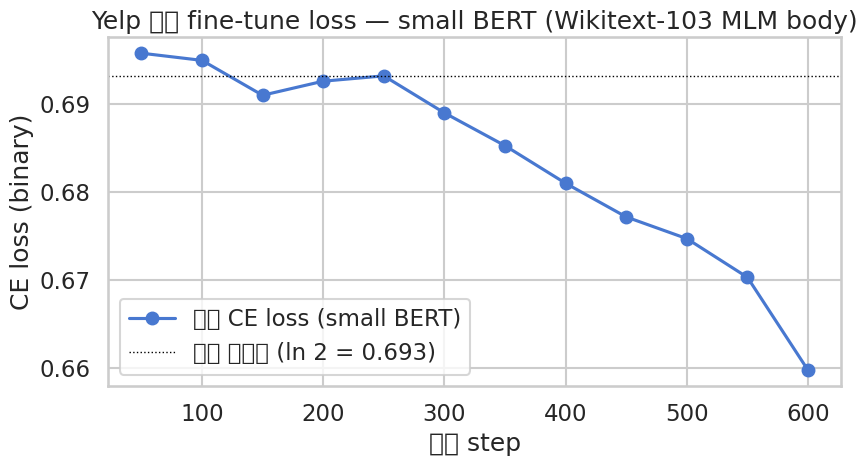
\includegraphics[width=0.82\linewidth]{assets/figures/ch21_finetune_loss.png}
\end{bookfigurelabel}

\textbf{그림 읽기} --- 그림~\ref{fig:ch21-finetune-loss}에서 다음 내용을 확인합니다: 작은 BERT의 Yelp 이진 분류 fine-tune loss 곡선. 실행된 노트북에서 저장된 최신 plot 출력이므로, 코드에서 계산한 값이 어떤 평가 지점으로 이어지는지 바로 확인할 수 있습니다.



\subsection{혼동 행렬}



\compactCodeOmitted{예측 결과를 지표와 표로 요약하는 단계}

\begin{bookfigurelabel}[H]{작은 BERT의 Yelp 이진 분류 혼동 행렬}{fig:ch21-confusion-matrix}
\centering
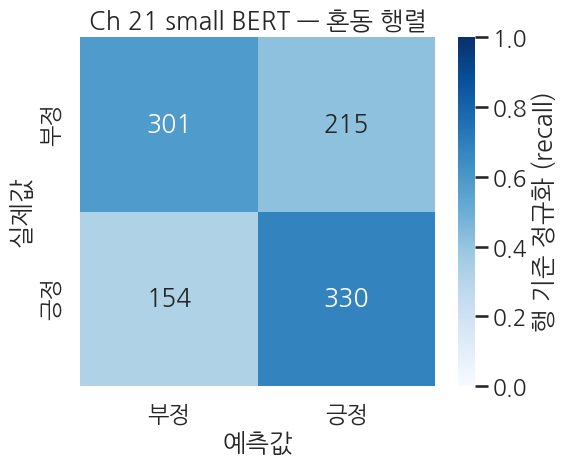
\includegraphics[width=0.68\linewidth]{assets/figures/ch21_confusion_matrix.png}
\end{bookfigurelabel}

\textbf{그림 읽기} --- 그림~\ref{fig:ch21-confusion-matrix}에서 다음 내용을 확인합니다: 작은 BERT의 Yelp 이진 분류 혼동 행렬. 실행된 노트북에서 저장된 최신 plot 출력이므로, 코드에서 계산한 값이 어떤 평가 지점으로 이어지는지 바로 확인할 수 있습니다.



\section{\ref{ch:10}장 (DistilBERT) vs \ref{ch:21}장 (작은 BERT scratch) --- 본 장의 핵심 결과}

\emph{같은 데이터·같은 hyperparams} 에 \emph{본체 출발점만 다른} 두 셋업의 정확도 비교. 둘 다 \emph{일반 도메인 위키 사전학습 \(\to\) Yelp 분류 transfer} 의 같은 패턴이라 비교가 \emph{fair}. \ref{ch:10}장의 수치는 본 장을 작성하는 시점에 \emph{해당 노트북의 README/실행 결과} 를 참고해 인용 --- 학습자가 노트북을 돌려 본인 수치로 갱신해 보면 더 좋습니다.

\begin{booktable}{21장 10장 (DistilBERT) vs 21장 (작은 BERT scratch) - 본 장의 핵심 결과 표}{tab:ch21-11}
\begin{adjustbox}{max width=\textwidth}
\begin{tabular}{@{}llll@{}}
\toprule
차원 & \ref{ch:10}장 (DistilBERT pretrained) & \ref{ch:21}장 (작은 BERT scratch + 2K \(\times\) 3 epoch MLM) & 비고 \\
\midrule

본체 파라미터 & 약 66M & 약 10M & \ref{ch:21}장은 1/6 크기 \\
사전학습 코퍼스 & Wikipedia + BookCorpus (약 33억 토큰, 일반 도메인) & Wikitext-103 paragraphs 2K (약 27만 토큰, 일반 도메인) & 약 1.2만배 격차, \textbf{둘 다 일반 위키} \\
사전학습 시간 & TPU 수일 & \textbf{T4 약 15초} (2K \(\times\) 3 epoch = 198 step) & \\
Fine-tune 도메인 & Yelp 이진 (사전학습과 다른 도메인) & Yelp 이진 (사전학습과 다른 도메인) & \textbf{둘 다 일반 \(\to\) Yelp transfer} \\
분류 fine-tune 셋업 & (같음 --- 5K/1K, batch 16, lr 2e-5, 2 epoch, fp16) & & 본체 외 통제 \\
\bottomrule
\end{tabular}
\end{adjustbox}
\end{booktable}



\compactCodeOmitted{예측 결과를 지표와 표로 요약하는 단계}

\begin{bookfigurelabel}[H]{Yelp 이진 분류에서 DistilBERT와 작은 BERT 비교}{fig:ch21-ch10-compare}
\centering
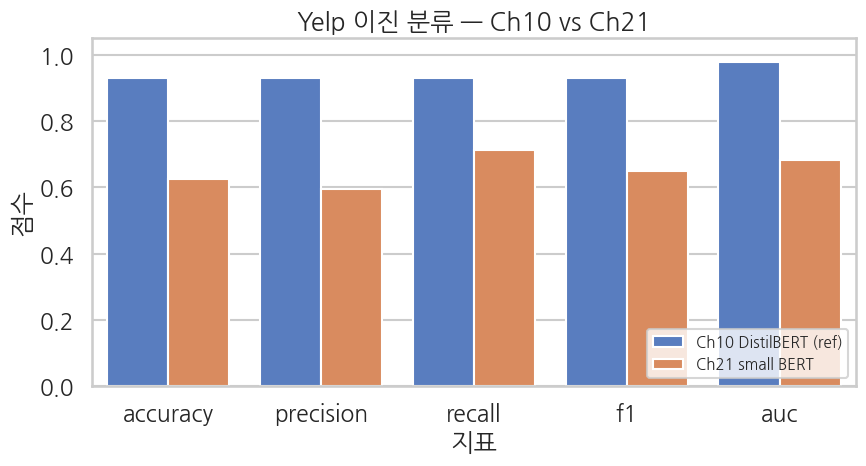
\includegraphics[width=0.82\linewidth]{assets/figures/ch21_ch10_compare.png}
\end{bookfigurelabel}

\textbf{그림 읽기} --- 그림~\ref{fig:ch21-ch10-compare}에서 다음 내용을 확인합니다: Yelp 이진 분류에서 DistilBERT와 작은 BERT 비교. 실행된 노트북에서 저장된 최신 plot 출력이므로, 코드에서 계산한 값이 어떤 평가 지점으로 이어지는지 바로 확인할 수 있습니다.



\textbf{관찰 --- \emph{동일 transfer 패턴 안에서 약 1.2만배 사전학습 격차} 가 분류 정확도에 어떻게 드러나나}

실측 (실행본 기준 \emph{근사}):

\begin{itemize}
\tightlist
\item
  \ref{ch:10}장 (DistilBERT, 대규모 Wiki+BookCorpus 사전학습): accuracy 약 0.90, AUC 약 0.97
\item
  \ref{ch:21}장 (작은 BERT, Wikitext-103 2K paragraphs \(\times\) 3 epoch 사전학습): \textbf{위 비교 셀 출력이 이번 실행의 값} --- random (0.50) 은 뚜렷이 넘지만 \ref{ch:10}장에는 크게 못 미칩니다
\end{itemize}

\textbf{accuracy 격차가 20\%p 를 훌쩍 넘습니다.} 두 모델이 \emph{같은 transfer 패턴} (일반 위키 \(\to\) Yelp) 을 따르므로 이 격차의 거의 전부가 \emph{사전학습 규모의 가치} --- Wikipedia + BookCorpus 약 33억 토큰의 \emph{일반 영어 지식} 이 DistilBERT 본체에 압축되어 있어, Yelp 같은 \emph{다른 도메인} 에도 빠르게 적응합니다.

\begin{quote}
\textbf{왜 \emph{약} 으로 적나} --- 위 수치는 \emph{실행본 한 판의 기록} 입니다. 이 장은 \textbf{무엇이 그 흔들림을 만드는가} 를 실험으로 확인한 자리이기도 합니다.

처음에는 \inlinecode{TrainingArguments(seed=42)} 만 걸려 있었습니다. 그때 \emph{같은 코드, 같은 날, 같은 라이브러리} 로 돌린 판들이 accuracy \inlinecode{0.6150} 부터 \inlinecode{0.6990} 까지 벌어졌습니다 --- 8\%p 가 넘는 폭입니다. 원인은 \textbf{모델 가중치의 random init} 이었습니다. \inlinecode{TrainingArguments} 의 \inlinecode{seed} 는 Trainer 가 학습을 시작한 뒤부터 적용되므로, 그 전에 만들어지는 본체와 분류 헤드의 초기값은 매번 달랐습니다.

지금은 모델 생성 직전마다 \inlinecode{set\_seed(SEED)} 를 겁니다 (§4-1 · §5 셀). 같은 커밋으로 연달아 돌린 두 판이 accuracy \inlinecode{0.6320} / \inlinecode{0.6310}, eval loss \inlinecode{0.6613} / \inlinecode{0.6610}, MLM perplexity \inlinecode{1368.18} / \inlinecode{1368.41} 로 \textbf{마지막 자리에서만 갈립니다.} 흔들림의 대부분은 fp16 연산 순서가 아니라 \emph{초기값} 이었던 셈입니다.

남은 0.1\%p 수준의 차이가 fp16 연산 순서·cuDNN 커널 선택에서 오는 몫입니다. 반면 파라미터 수 (\inlinecode{11,103,290}) 와 block 수 (\inlinecode{2,100}) 는 \textbf{어느 판에서도 같습니다.} \emph{설정에서 결정되는 값은 완전히 재현되고, 학습을 거친 값은 마지막 자리가 흔들립니다.} 그래서 이 장은 앞의 것만 정확값으로 적고, \textbf{학습 metric 은 셀 출력을 단일 출처로 두고 본문에서 숫자를 못 박지 않습니다} --- 시드를 걸어도 라이브러리 버전이 올라가면 이 정도 재현성은 다시 흔들리기 때문입니다. 여러분이 직접 돌린 값이 실행본과 조금 달라도 정상입니다.
\end{quote}

\begin{quote}
한편 \ref{ch:21}장의 accuracy 가 \emph{random (50\%) 보다 훨씬 높다} 는 것도 중요한 결과입니다. 작은 일반 도메인 사전학습 + 작은 모델로도 \emph{기본 위키 어휘·문맥 구조} 가 본체에 들어가 Yelp 분류의 \emph{기본 신호} (긍정/부정 단어들의 통계) 가 잡힙니다.
\end{quote}



\section{참고: fair-compute 비교}

\emph{MLM 사전학습 없이 random init 으로 바로 분류 fine-tune}, 그리고 \emph{같은 GPU compute budget (MLM 시간 + fine-tune 시간 합)} 으로 \emph{분류 fine-tune 만 더 길게} 돌렸을 때 어떻게 되는지는 부록 노트북 \href{https://colab.research.google.com/github/yoon-gu/neuqes-101/blob/master/21_en_bert_classify/appendix_compute_budget.ipynb}{\inlinecode{appendix\_compute\_budget.ipynb}} 에서 다룹니다.

\begin{quote}
부록의 핵심 질문 --- \emph{“사전학습에 쓰는 compute 를 단순히 fine-tune 에 더 쓰면 안 되나?”} 에 대한 정량 답. \textbf{이 규모에서는 \textquotesingle 그래도 된다\textquotesingle{} 가 답입니다} --- 부록 실측에서 fair-compute 셋업이 사전학습 셋업을 앞섭니다. 사전학습이 이기려면 \ref{ch:10}장 급 \emph{규모} 가 필요하다는 것을 반대편에서 보여 줍니다.
\end{quote}



\section{이 장에 등장한 라이브러리·함수}

\begin{booktable}{21장 새로 등장한 라이브러리}{tab:ch21-12}
\begin{adjustbox}{max width=\textwidth}
\begin{tabular}{@{}lll@{}}
\toprule
이름 & 한 줄 설명 & 다음 장에서 \\
\midrule

\inlinecode{transformers.BertForSequenceClassification} & encoder + 분류 head, 분류 fine-tune 전용 & \ref{ch:23}장 한국어 분류 \\
\inlinecode{BertForSequenceClassification(config)} (random init) & pretrained weight 없이 모델 생성 & \ref{ch:23}장 같음 (random baseline) \\
\inlinecode{model.bert.load\_state\_dict(other.bert.state\_dict())} & 본체만 통째로 옮기는 in-memory 헤드 교체 & \ref{ch:23}장 같음 \\
\inlinecode{transformers.BertForMaskedLM} (재등장) & MLM 사전학습 (\ref{ch:20}장 압축 재현) & \ref{ch:22}장 한국어 MLM \\
\inlinecode{load\_dataset("Salesforce/wikitext",\ "wikitext-103-raw-v1")} & Wikitext-103 일반 도메인 코퍼스 로드 (MLM 용) & \ref{ch:22}장 한국어 Wikipedia 패턴과 대칭 \\
\inlinecode{load\_dataset("fancyzhx/yelp\_polarity")} & Yelp 이진 분류 데이터 (분류 fine-tune 용) & \ref{ch:23}장 NSMC 와 대칭 \\
\inlinecode{sklearn.metrics.precision\_recall\_fscore\_support(...,\ average="binary")} & 이진 분류 metric 한 묶음 & \ref{ch:23}장 동일 \\
\inlinecode{sklearn.metrics.roc\_auc\_score} & AUC & \ref{ch:23}장 동일 \\
\bottomrule
\end{tabular}
\end{adjustbox}
\end{booktable}



\section{체크포인트 질문}

\begin{enumerate}
\def\labelenumi{\arabic{enumi}.}
\tightlist
\item
  \inlinecode{BertForMaskedLM} 과 \inlinecode{BertForSequenceClassification} 둘 다 \emph{내부에 같은 \inlinecode{BertModel}} 을 갖습니다. 두 모델 사이에서 \emph{어떤 파라미터} 가 이어지고 \emph{어떤 파라미터} 가 새로 학습되나요?
\item
  MLM 학습 첫 step 의 loss 가 약 10.33 인 반면, 분류 fine-tune 첫 step 의 loss 는 약 0.693 입니다. 이 \emph{4 배 차이} 가 모델의 학습 어려움 차이를 의미하나요? (힌트: K=vocab\_size vs K=2)
\item
  \ref{ch:21}장의 작은 BERT 가 \ref{ch:10}장의 DistilBERT 보다 \emph{낮은 정확도} 를 보입니다. 이 격차가 (a) \emph{모델 크기} 차이 (약 10M vs 약 66M), (b) \emph{사전학습 데이터 양} 차이 (약 27만 토큰 vs 약 33억 토큰) 중 어느 쪽 영향이 클까요? 둘 다 \emph{위키 일반 도메인 \(\to\) Yelp transfer} 의 같은 패턴이라 \emph{도메인 정합} 변수는 통제됨. 추가 실험으로 어떻게 (a) 와 (b) 를 분리할 수 있나요?
\item
  \emph{MLM 3 epoch} 와 \emph{random init} baseline 의 정확도 차이가 매우 작거나 (예: 1-2\%p) 거꾸로 \emph{random 이 더 높게} 나올 가능성이 있나요? 어떤 상황에서 그럴 수 있을까요? (힌트: 한국어 \ref{ch:23}장 부록 참조)
\end{enumerate}



\section{FAQ}


\begin{faqBox}{Q2. (이론) 왜 \emph{task 도메인 (Yelp) 자체로} 사전학습하지 않고 일반 위키 (Wikitext-103) 로 사전학습하나요? 같은 도메인에서 학습한 게 transfer 가 더 유리하지 않나요?}

같은 도메인 사전학습 \(\to\) 같은 도메인 fine-tune 은 \emph{domain-adaptive pretraining} (DAPT) 에 더 가깝습니다 --- \emph{사전학습이 이미 task 도메인의 표현} 을 학습한 상태에서 분류만 얹는 셈. \emph{정직한 transfer 측정} 이 아닙니다.

\Needspace{5\baselineskip}
\begin{lstlisting}

\end{lstlisting}

본 장의 \emph{\ref{ch:10}장 vs \ref{ch:21}장} 비교가 \emph{공정} 한 이유 --- 둘 다 \emph{일반 도메인 위키 사전학습 \(\to\) Yelp 분류} 의 같은 패턴이라 \emph{사전학습 규모} (약 1.2만배) 와 \emph{모델 크기} (약 6배) 만 변수. 만약 \ref{ch:21}장이 Yelp 사전학습이었다면 \emph{어느 효과가 격차를 만들었는지} 분리할 수 없었을 것.

\begin{quote}
\ref{ch:22}--\ref{ch:23}장 (한국어 위키 \(\to\) NSMC 영화 리뷰) 도 \emph{같은 대칭 패턴}. \emph{일반 도메인 \(\to\) 다른 도메인 transfer} 가 사전학습-fine-tune 패러다임의 \emph{진짜 메시지}.
\end{quote}

\end{faqBox}

\begin{faqBox}{Q3. (이론) MLM 본체 가중치를 \emph{완전히 같은} hyperparams 에 옮겼는데 왜 분류 정확도가 \emph{작은 폭} 만 개선되나요?}

\textbf{작은 데이터의 한계} --- 사전학습 코퍼스 (Wikitext-103 paragraphs 2K = 약 27만 토큰) 자체가 \emph{학습할 언어 분포} 가 좁습니다. DistilBERT 의 사전학습 코퍼스 (약 33억 토큰) 와 비교하면 약 1.2만배 작은 데이터로 같은 일을 한 것.

\Needspace{6\baselineskip}
\begin{lstlisting}
mlm_train_raw = (
    raw_train.filter(is_good).shuffle(seed=SEED).select(range(20000))
    .remove_columns([c for c in raw_train.column_names if c != "text"])
)
\end{lstlisting}

실측 기준 2K \(\times\) 3 epoch 학습이 약 15초이므로, \inlinecode{N\_MLM\_TRAIN} 을 열 배 늘려도 학습 자체는 2-3분 수준입니다 (T4 30분 룰에 먼저 걸리는 쪽은 학습이 아니라 \emph{다운로드·전처리}). 그래도 \emph{대규모 사전학습} 의 격차는 메우기 어렵습니다 --- \emph{데이터 규모 자체의 가치} 가 진짜 BERT 의 비밀.

\end{faqBox}

\begin{faqBox}{Q4. (실무) MLM 사전학습이 fine-tune 정확도에 \emph{해가 되는} 경우가 있나요?}

드물지만 있습니다. 두 가지 시나리오:

\Needspace{5\baselineskip}
\begin{lstlisting}
MLM_EPOCHS = 20
\end{lstlisting}

(1) 의 경우 본체가 \emph{특정 문장 패턴에 과적합} 되어 fine-tune 일반화가 떨어질 수 있습니다. \emph{MLM eval loss} 와 \emph{MLM train loss} 의 격차로 진단 --- 격차가 커지면 overfitting.

(2) 의 경우 본체가 \emph{downstream 도메인에 무관한 표상} 을 학습. 토크나이저까지 안 맞으면 거의 동작 안 함 (\ref{ch:19}장의 cross-language 실험). 본 장처럼 \emph{위키 영어 \(\to\) Yelp 영어} 는 \emph{도메인은 달라도 같은 언어 + 어휘 일부 공유} 라 transfer 가 작동.

\end{faqBox}







\compactFAQMore{5}

\begin{previewBox}{미리보기: 다음 장}

\textbf{\ref{ch:22}장. 작은 BERT 직접 사전학습 --- 한국어 MLM (scratch, 한국어 Wikipedia)}

\begin{itemize}
\tightlist
\item
  \ref{ch:20}장의 영어 패턴을 한국어로 그대로: 작은 BertConfig + \inlinecode{klue/bert-base} 토크나이저 (가져옴) + \textbf{한국어 Wikipedia paragraphs MLM} (일반 도메인)
\item
  토크나이저·데이터만 한국어로 바뀜. 본체 구조·MLM 셋업은 \emph{완전히 같음}
\item
  \ref{ch:22}장 \(\to\) \ref{ch:23}장 (한국어 NSMC 분류) 흐름은 본 장 (\ref{ch:20}장 \(\to\) \ref{ch:21}장, 영어) 와 \emph{대칭} --- 둘 다 \emph{일반 위키 사전학습 \(\to\) 다른 도메인 분류 transfer} (영어는 Yelp 리뷰(식당·업체), 한국어는 NSMC 영화 리뷰)
\end{itemize}

\begin{quote}
\textbf{변하는 축}: Phase 3 안에서 \emph{언어} (영어 \(\to\) 한국어). 모델 구조·학습 셋업·\emph{일반 도메인 \(\to\) task 도메인 transfer 패턴} 은 동일.
\end{quote}

본 장 (\ref{ch:21}장) 에서 본 \emph{일반 위키 사전학습 + 다른 도메인 분류 transfer} 의 격차 패턴이 \ref{ch:23}장에서 \emph{한국어 환경} 에서도 같은 결을 그리는지 확인하는 게 Phase 3 의 마지막 메시지.
\end{previewBox}